\subsection{Clustering}
\label{Res_Clu}
We cluster the data into five clusters. Assuming equal distribution of nations into the clusters, we will have \begin{math}\frac{30}{5} = 6\end{math} nations in each cluster in a year.

Running the Weka's simpleKMeans clustering algorithm with \textit{numberOfClusters} set to 5 results in the graph displayed on page \pageref{fig:clusters} (figure \ref{fig:clusters})\footnote{A larger version is illustrated by figure \ref{fig:largeClusters} on page \pageref{fig:largeClusters} in the appendix.}.
\\The x-axis are the different European nations, the y-axis are the years and the colour is the cluster the country/year combination belongs to.

\begin{figure}[h!]
  \centering
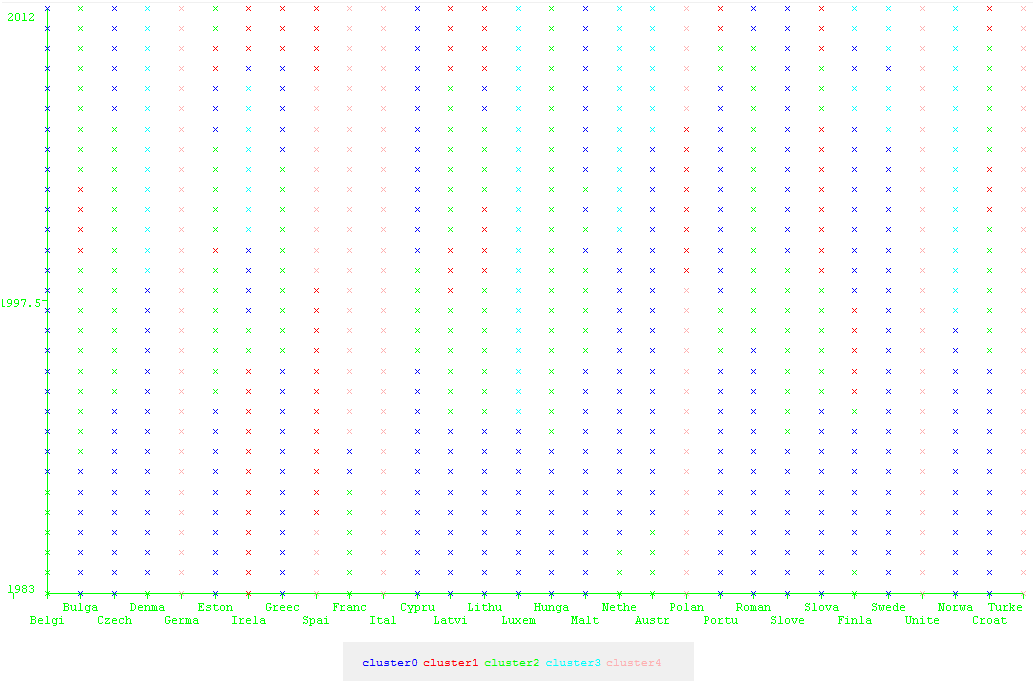
\includegraphics[width=\textwidth]{Appendix/Images/kMeans}
\caption{Graphical representation of what clusters the countries belong to at what year}
\label{fig:clusters}
\end{figure}

There are four nations that never change cluster: Germany, Italy, Turkey and the United Kingdom. Interestingly all four of them are in the same cluster (cluster\#4). This is likely due to their population being quite comparable\footnote{Russia has a far higher population than the four mentioned countries and so it is not likely to be a stable part of that cluster.}\footnote{France has a somewhat comparable population size, so this is not necessarily the case.}.

The other extreme are the countries changing clusters often. In this case we define \textit{often}\footnote{We feel that any nation changing clusters more often than every 4 years on average is quite unstable.} as 
\begin{align*}
often = \frac{number of years}{4} = \frac{30}{4} = 7,25 \sim 7
\end{align*} 
\\There is only one nation that changes cluster seven times or more: Finland. Estonia and Malta are close contenders with 6 cluster changes. It is interesting to note that all three countries are somewhat stable for much of 1983-2012 but with some periods where they change clusters often:

\begin{itemize}
\item Finland starts in cluster \#2 (1983), but changes to cluster \#0 in 1985 and stays there until 1991 where it goes back to cluster \#2. Finland then spends five years in cluster \#1 (1992-1996), after which it goes back to cluster \#0 for 9 years (1997-2006). In 2007 it changes to cluster \#3 (2007-2008) then spends two years in cluster \#0 (2009-2010) and the remaining two years in cluster \#3. 
\item Estonia starts in cluster \#0 (1983-1992), then changes to cluster \#2 for a while (1993-1999 \& 2001-2005) with one year in cluster \#1 (2000). It is in cluster \#0 during (2006-2008) then spends two years in cluster \#1 (2009-2010) closing off with two years in cluster \#2 from 2011 to 2012.
\item Malta starts in cluster \#0 (1983-1994) then changes to cluster \#2 for five years (1995-1999). It is in cluster \#0 in 2000 and 2002 with two single years in cluster \#2 (2001 \& 2003). It is in cluster \#0 for the rest of the period.
\end{itemize}

Injecting the United States of America (2011) into the clusters\footnote{For Weka output, see appendix section \ref{A_kmr_usa} on page \pageref{A_kmr_usa}.} puts USA into cluster \#4. Worthy of note is that cluster \#4 is also the cluster containing Germany, Italy, Turkey and the United Kingdom. Going by this clustering alone, one could argue that USA of 2011 is - economically speaking - more like these four countries that any other European countries.

\subsubsection*{Correctness}
\label{Res_Clu_Cor}
While the value of "Within cluster sum of squared errors"\footnote{The lower the value of "Within cluster sum of squared errors", the closer the elements of the cluster is to the cluster centroid.} is somewhat low considering our quite attribute high values (compared to the SEE value), we still feel that our results are unreliable. Because the simpleKMeans uses Euclidean distance to compare elements, the non-normalised value of population is much more impactful than unemployment rate, thus skewering the data in a way we had not intended.